\section{Velvet FlyClient}
\label{sec:flyclient}
In the FlyClient paper~\cite{flyclient} a velvet fork is suggested for the deployment of the protocol as-is, 
followed by a short argument for its respective security. In this document we describe an explicit attack against 
the FlyClient protocol under velvet fork deployment. 
This is essentially a kind of ``Chainsewing Attack''.

\subsection{The FlyClient Protocol}
	The FlyClient protocol suggests that block headers additionaly include an MMR root of all the blocks in the chain. The protocol uses this root hash in multiple ways, both for chain synchronization and specific block queries. Consider a block $b$ which is appended to the chain $\chain$ at height $h_b$: 
	\begin{itemize}
		\item the prover generates a merkle inclusion proof $\Pi_b$ for the existence of $b$ at height $h_b$ in $\chain$ with respect to the MMR root included in the \emph{head} or \emph{tip} of the chain $\chain[-1]$
		\item the verifier receives the merkle root of the chain from a prover and an inclusion proof $\Pi_b$ for block $b$. He also generates from $\Pi_b$ the root of the MMR subtree of all blocks in $\chain$ from genesis up to $\chain[h_b - 1]$ and verifies that it is equal to the merkle root included in the header of block $b$.
	\end{itemize}
	The above proofs are produced with respect to the MMR root included in $\chain[-1]$.

	\vspace{2mm}
	\noindent
	A high level description of the FlyClient is as follows. Suppose that  the verifier, a superlight client, asks to synchronize to the current longest valid chain.  Suppose that he receives different proofs from two provers. Each prover sends (the header) of the last block in the chain, $\chain[-1]$, and a claim for the number of blocks in his chain, $\lvert \chain \rvert$. If both proofs are valid, then the one claiming the greater block count is selected. The validity check of a proof goes as follows. 
	The verifier has received $\chain[-1]$, $\lvert \chain \rvert$ and queries $k$ random block headers from each prover based on a specific probabilistic sampling algorithm. For each queried block $B_i$ the prover sends the header of $B_i$ along with an MMR subtree inclusion proof $\Pi_{B_i}$ that $B_i$ is the $i_\text{th}$ block in the chain. The verifier also checks that $B_i$ is normally mined on the same chain as $\chain[-1]$ by verifying that the root included in $B_i$ is the MMR root of the first ($\lvert \chain \rvert - 1$) blocks' subtree. If the $k$ random sampled blocks successfully pass through this verification procedure then the proof is considered valid, otherwise the proof is rejected by the verifier. 
	The chain synchronization protocol is given in Algorithm~\ref{alg:flyclient_suffix_protocol}.

	\begin{algorithm}[h]
		\caption{\label{alg:flyclient_suffix_protocol}FlyClient protocol~\cite{flyclient}}
		A client (i.e the Verifier) performs the following steps speaking with two provers who want to convince him that they hold a valid chain of length $n+1$. At least one of the provers is honest. If the provers claim different length for their claims then the longer chain is checked first.
		\begin{enumerate}
			\item The provers send to the verifier the last block header in their chain. Each header includes the root of an MMR created over the first $n$ blocks of the corresponding chain. 
			\item The verifier queries $k$ random block headers from each prover based on the described optimal probabilistic sampling algorithm.
			\item For each queried block, $B_i$, te prover sends the header of $B_i$ along with an MMR proof $\Pi_{B_i \in \chain}$ that $B_i$ is the $i-$th block in the chain.
			\item The client performs the following checks for each block $B_i$ according to Algorithm  and rejects the proof if any checks fail
			\item The client rejects the proof if any checks fail
			\item Otherwise, the client accepts $\chain$ as the valid chain
		\end{enumerate}
	\end{algorithm}

	\begin{algorithm}[h!]
		\caption{\label{alg:flyclient_iinfix_protocol}Prover/Verifier protocol for a single query~\cite{flyclient}}
		The verifier queries the prover for the header and MMR proof for a single block $k$ in the prover's chain of $n+1$ blocks.
		\begin{center}
			\textbf{Verifier}
		\end{center}
		\begin{enumerate}
			\item Has the root of the MMR of $n$ blocks stored in the $n+1$ block's header 
			\item Queries prover for the header of block $k$ and for $\Pi_{k \in n}$
			\item Verifies that the hashes of $\Pi_{k \in n}$ hash up to the root of MMR$_n$
			\item Calculates the root of the MMR of the $k-1$ blocks from $\Pi_{k \in n}$ 
			\item Compares the calculated root with the root in the header of block $k$
			\item If everything checks out, accepts the block proof
		\end{enumerate}
		\begin{center}
			\textbf{Prover}
		\end{center}
		\begin{enumerate}
			\item Has chain of $n+1$ blocks and the MMR of the first $n$ blocks 
			\item Receives query for block $k$ from verifier 
			\item Calculates $\Pi_{k \in n}$ from MMR$_n$
			\item Sends header of $k$ and $\Pi_{k \in n}$ to verifier
		\end{enumerate}
	\end{algorithm}

	For a single block query the protocol can be described as follows. The verifier is synchronized to a chain $\chain$ and already has the tip of the chain $\chain[-1]$. He then queries the prover and receives the header of the specific block of interest $B$ in $\chain$ and the inclusion proof $\Pi_{B \in \chain}$. Then the verifier checks the validity of $B$ in the same way as already described for the random sampled blocks in the synchronization protocol. 
	The prover/verifier single-query protocol is given in Algorithm~\ref{alg:flyclient_iinfix_protocol}.


\subsection{Velvet MMRs}
	A velvet fork suggests that any protocol changes are deployed in a backwards-compatible manner so that unupgraded players accept upgraded blocks and upgraded players accept unupgraded blocks too. In practice, the protocol changes are applied via some auxiliary data included in each block, which make sense and are used only by upgraded parties,while being omitted as comments by unupgraded parties. 

	In the context of FlyClient, velvet fork deployment implies that upgraded miners additionally include an MMR root in each block's header. 
    The claim made in the paper is that considering a constant fraction $\alpha$ of upgraded blocks in the chain, an honest prover could produce proofs 
    by utilizing only these blocks and by joining the intermediary blocks together. 
    The claim is that the velvet proofs remain secure. We believe that the velvet protocol is susceptible to a kind of chainsewing attack, which shall succeed with non-negligible probability.
    In the following we describe this attack and leave the analysis for future work. 

	Velvet fork requires any block to be accepted in the chain regardless the validity of the auxiliary data coming with the protocol update. 
    In the case of FlyClient, an adversary may produce blocks which are compatible to the basic consensus rules but contain invalid MMR information. 
    As an example, consider an invalid MMR that omits blocks existing in $\chain$ or contain blocks which belong in temporary forks of $\chain$. 
    We call adversarially generated blocks containing invalid MMRs \emph{thorny} blocks. A specific case of thorny is illustrated in Figure~\ref{fig:thorny_flyclient}.

	\begin{figure}
		\begin{center}
			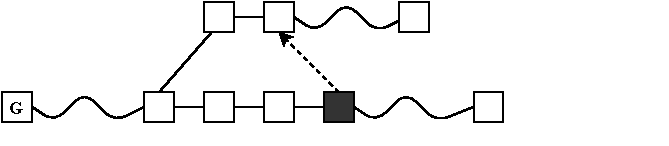
\includegraphics[width=0.5\columnwidth]{figures/false_interlink.pdf}
		\end{center}
		\caption{A thorny block, colored black, containing invalid MMR commitment to a block of a fork chain illustrated as a dashed arrow. With respect to the MMR commitments the black block along with the grey ones form a chain.}
		\label{fig:thorny_flyclient}
	\end{figure}


\subsection{The Attack}
	The  velvet FlyClient description has not examined the case of thorny blocks, i.e. blocks that contain only seemingly valid auxiliary data, and their impact on the protocol's overall security.
	At this point we have to make two assumptions considering thorny blocks in FlyClient:
	\begin{enumerate}
		\item honest miners validate the MMR root of the blocks and treat thorny blocks as unupgraded
		\item the number of random sampled \emph{upgraded} blocks is of importance for the verifier's decision regarding the valid chain. The verifier should accept the proof that delivers the most upgraded blocks.
	\end{enumerate}
    The first assumption is obviously reasonable. In the opposite case any block containing trash data in the place where the MMR root would be able to 
    completely destroy the protocol making it impossible to deliver a valid proof.
	Regarding the second assumption let us show that the protocol is trivially attackable in the opposite case. Consider an attacker who acts as follows.
	Consider three consecutive blocks in the honest chain $b_i$, $b_{i+1}, b_{i+2}$ at height $i, i+1, i+2$ respectively. The attacker produces a thorny block $b'_{i+1}$ on top of $b_i$ containing a double spend transaction in conflict with $b_{i+1}$. 
	Whenever she wants to convince a client that the honest chain contains $b'_{i+1}$ she produces another thorny block $b_j$ on top of the current chain's tip and sends her proof. Note that $b_j$ contains an MMR that considers 
	$b'_{i+1}$, but also that her thorny blocks are the only possible upgraded blocks in her proof. More specifically $b_j$ will appear in the proof as it is the tip of the chain, while $b_{i+1}$ will be in the proof 
	only if it is selected by the random sampler. Her proof will only be found invalid if the random sampler queries both blocks at heights $i+1, i+2$, so that the invalid prevId pointer shows up. The attacker can decrease this probability
	by letting the chain grow enough before attempting to construct a proof, as the random sampler chooses older blocks with lower probability. It is now obvious that the verifier will most probably receive two valid proofs of the same length, one from the attacker and one from an honest node.
	If the number of upgraded blocks appearing in the proof are not to be considered then this attack succeeds with high probability even for an adversary of low hashing power.
	Note that the above assumptions are in favor of the protocol. 

	We will now describe the chainsewing attack against the velvet FlyClient protocol under these asumptions.

	Consider that the adversary utilizes more than one thorny blocks, in order to cut-and-paste portions from the chain adopted by honest parties to his fork chain. 
	%Consider the attack illustrated in Figure~\ref{fig:simple_chainsewing_flyclient}. 
    The adversary acts as follows. 
    She first mines upgraded blocks on a fork chain $\chain_A$ until she generates block $b'$ containing a double spending attack. 
    Afterwards she mines block $a'$ in the honest chain $\chain_B$, which includes an MMR root for her fork chain, thus including the blocks from genesis and up to $b'$. 
    Next she keeps mining blocks on $\chain_B$, which contain MMR root that builds on top of the root included in $a'$. While constructing the MMRs of her blocks she considers only her 
    adversarial blocks and ignores any intermediary honest blocks. 
    Additionally, during this period when she mines on $\chain_B$ she tries to suppress any honest upgraded block in $\chain_B$ by mining selfishly. 
    In essence, she regularly mines block on $\chain_B$ as described excluding honestly unupgraded blocks from the MMRs. 
    When an honest upgraded block $\chain[i]$ is appended she mines on top of block $\chain[i-1]$. 
    Even if she mines a block and the suppression fails she can still use her fresh block in her proof by continuing to construct consistent MMRs 
    in the coming blocks as described before. Figure~\ref{fig:combined_chainsewing_flyclient} illustrates an example of the underlying suppression attack.
	From the verifier's perspective the ignored honest blocks are simply perceived as unupgraded blocks. At some later point, the adversary generates block $a$ 
    in the fork chain, which also contains an MMR root for all the grey and black blocks up to block $b$. 
    Right afterwards the adversary produces a proof as described in the velvet FlyClient protocol giving block $a$ as $\chain[1]$ 
    and the count number of all the grey and black blocks. From the verifier's perspective the black and grey colored blocks form a valid chain, 
    since the head of the chain $a$ contains consistent MMR commitments with all these blocks. 
    In addition, the random sampling performed by the FlyClient protocol will succeed because there are no invalid blocks in this chain.

%	\begin{figure}
%		\begin{center}
%			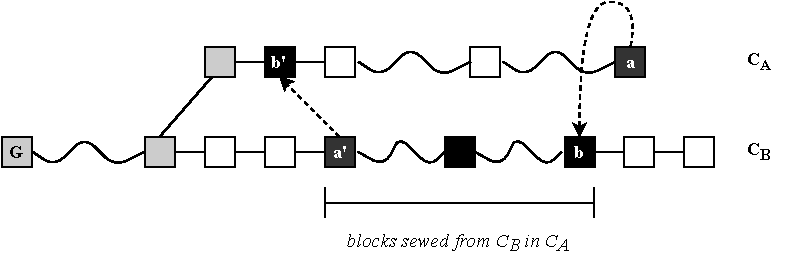
\includegraphics[width=0.95\columnwidth]{figures/simple_chainsewing_flyclient.pdf}
%		\end{center}
%		\caption{Chainsewing attack. Two thorny blocks $a, a'$ are used to chainsew a portion of honest chain $\chain_B$ to adversarial fork $\chain_A$. Black blocks imply adversarially generated blocks. Grey blocks are used in the adversarial proof along with the black ones. Wavy lines imply one or more blocks. Dashed arrows imply an MMR commitment for the destination block in the block of origin.}
%		\label{fig:simple_chainsewing_flyclient}
%	\end{figure}

	\begin{figure}
		\begin{center}
			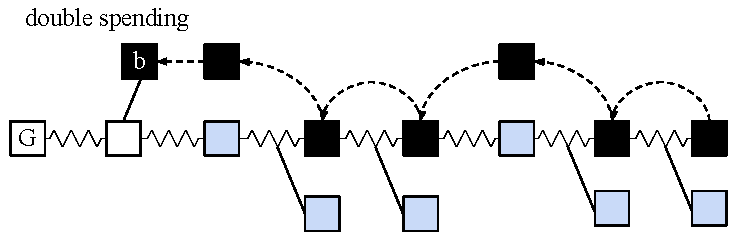
\includegraphics[width=0.8\columnwidth]{figures/attack_after_update-crop.pdf}
		\end{center}
		\caption{Chainsewing along with suppression attack. Black blocks imply adversarially generated blocks. Blue blocks imply honest upgraded blocks,which the adversary tries to suppress. Wavy lines imply one ore more blocks. Dashed arrows imply an MMR commitmens.}
		\label{fig:combined_chainsewing_flyclient}
	\end{figure}